\documentclass[12pt]{article}
\usepackage{geometry}
\geometry{a4paper, margin = 1in, left = 1.2in}
\usepackage{graphicx}
\graphicspath{{D:/Ze/Works/GitHub/Project2/Image/}}
\usepackage{float}
\usepackage{csvsimple}
\usepackage{pgfplotstable}
\usepackage{booktabs}

\begin{document}

\begin{titlepage}
	\begin{center}
		
		\LARGE{\bfseries DIY Automatic Delivery Trolley} \\
		[1cm]
		\normalsize by \\
		[1cm]
		Utchawin Namdee 5911697 \\
		Patipan Arunwattanawong 5912537 \\
		[1cm]
		A report submitted in partial fulfillment of the requirements for \\
		the degree of Bachelor of Engineering in \\
		Mechatronics Engineering \\
		[1cm]
		Project Advisor\\
		Asst. Prof. Dr. Narong Aphiratsakun \\
		[1cm]
		Examination Committee \\
		[1cm]
		Dr. Jerapong Rojanarowan, Dr. Wisuwat Plodpradista, \\
		Assoc. Prof. Dr. Jiradech Kongthon, Mr. Sunchanan Charanyananda, \\
		Mr. Amulya Bhattarai, Mr. Ehsan Ali \\
		[1cm]
		Assumption University \\
		Vincent Mary School of Engineering\\
		Thailand \\
		October 2020 \\
		
	\end{center}
\end{titlepage}

\newpage
\thispagestyle{empty}

\noindent Approved by Project Advisor:\newline
\hspace*{7cm} Name: Asst.Prof.Dr. Narong Aphiratsakun \\
\hspace*{7cm} Signature:\\
\hspace*{7cm} Date:\hrulefill \\
[1cm]
Plagiarism verified by: \\
\hspace*{7cm} Name: Mr. Ehsan Ali \\
\hspace*{7cm} Signature: \\
\hspace*{7cm} Date:\hrulefill \\

\newpage
\pagenumbering{roman}
\addcontentsline{toc}{section}{\numberline{}Abstract}

\section*{Abstract}\label{sec:abs}

\indent This project will describe the automatic delivery trolley for sending documents to a specific station. This system is able to deliver documents without human interaction using trolley mechanisms. Various type of documents can be sent/receive to and from several stations. Moreover, the trolley system can be control using command issue via mobile application. The system consists of infrared (IR) sensor to make the trolley run along the black line and ultrasonic sensor to avoid colliding with objects or people. This project can be used in various physical/environmental situations. For example, sending the documents or medicine in the hospital, homes with elderly or disabled people. In addition, the scale can be developed or expanded to use other works like transporting various parts in the factory or transportation between cities.

\newpage

\tableofcontents
\thispagestyle{empty}

\newpage
\pagenumbering{arabic}

\setcounter{page}{1}

\section{Introduction} \label{sec:intro}

\subsection{Introduction of Topic} \label{subsec:intro}

Nowadays, automation industrial plays significant role in the world as we can see in the daily life such as automatic door and vacuum cleaner robot. We can say that automation technology initiates other technology so that they have their own names and branch, for example, Robotics. We as a student would like to apply some automation technology to a daily life so that others can easily access to it. What we are going to do is DIY automatic delivery trolley.

\subsection{Project Objective} \label{subsec:project obj}

Delivery something to someone might be a hard time if there is far distant between them. So, we develop this DIY automatic delivery trolley to solve this problem. The user will use smart phone application to control the Trolley to deliver the item from one place to another.

\section{Project Overview} \label{sec:project over}

\subsection{Initial study \& Background study} \label{subsec:initial study}

Currently, there are many types of controller, but we found 2 main types of controller that are suitable for our project: Arduino and Raspberry Pi. \par
Raspberry Pi resembles a mini PC but use an OS that is developed from Linux. For the Raspberry Pi can use Python C++ to write the command. \par
Arduino is a microcontroller which can only work in accordance with the program that we wrote and there is no built-in OS. It is designed to be economical, small, does not require additional equipment for uploading sketches. there is also a port to connect with external sensors more than Raspberry Pi. There are various protocols which is a standard for connecting with external hardware for example I2C, SIP, UART including both Digital and Analog port. Importantly, it works more specifically type than Raspberry Pi for example real time control Arduino is more suitable than Raspberry Pi. In addition, Arduino is also designed the system to prevent over-voltage better than Raspberry Pi.

\section{System} \label{sec:system}

\subsection{Block diagram of the System} \label{subsec:block diagram}

\begin{figure}[H]
	\centering
	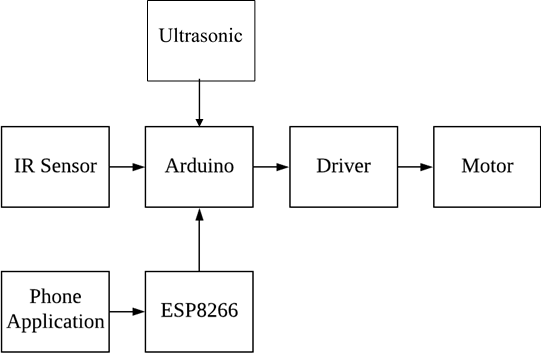
\includegraphics[height= 6cm]{Blockdiagram}
	\caption{Block diagram of the system} \label{fig:block}	
\end{figure}

The block diagram shown in Figure \ref{fig:block} depicts how our system works. Firstly, the microcontroller, Arduino, will receive the data from sensors and ESP8266. Then Arduino will send it to driver. Lastly, the driver will drive the motor.

\subsection{Controller} \label{sub:controller}

\subsubsection{Arduino Uno Board} \label{subsub:arduino}

\begin{figure}[H]
	\centering
	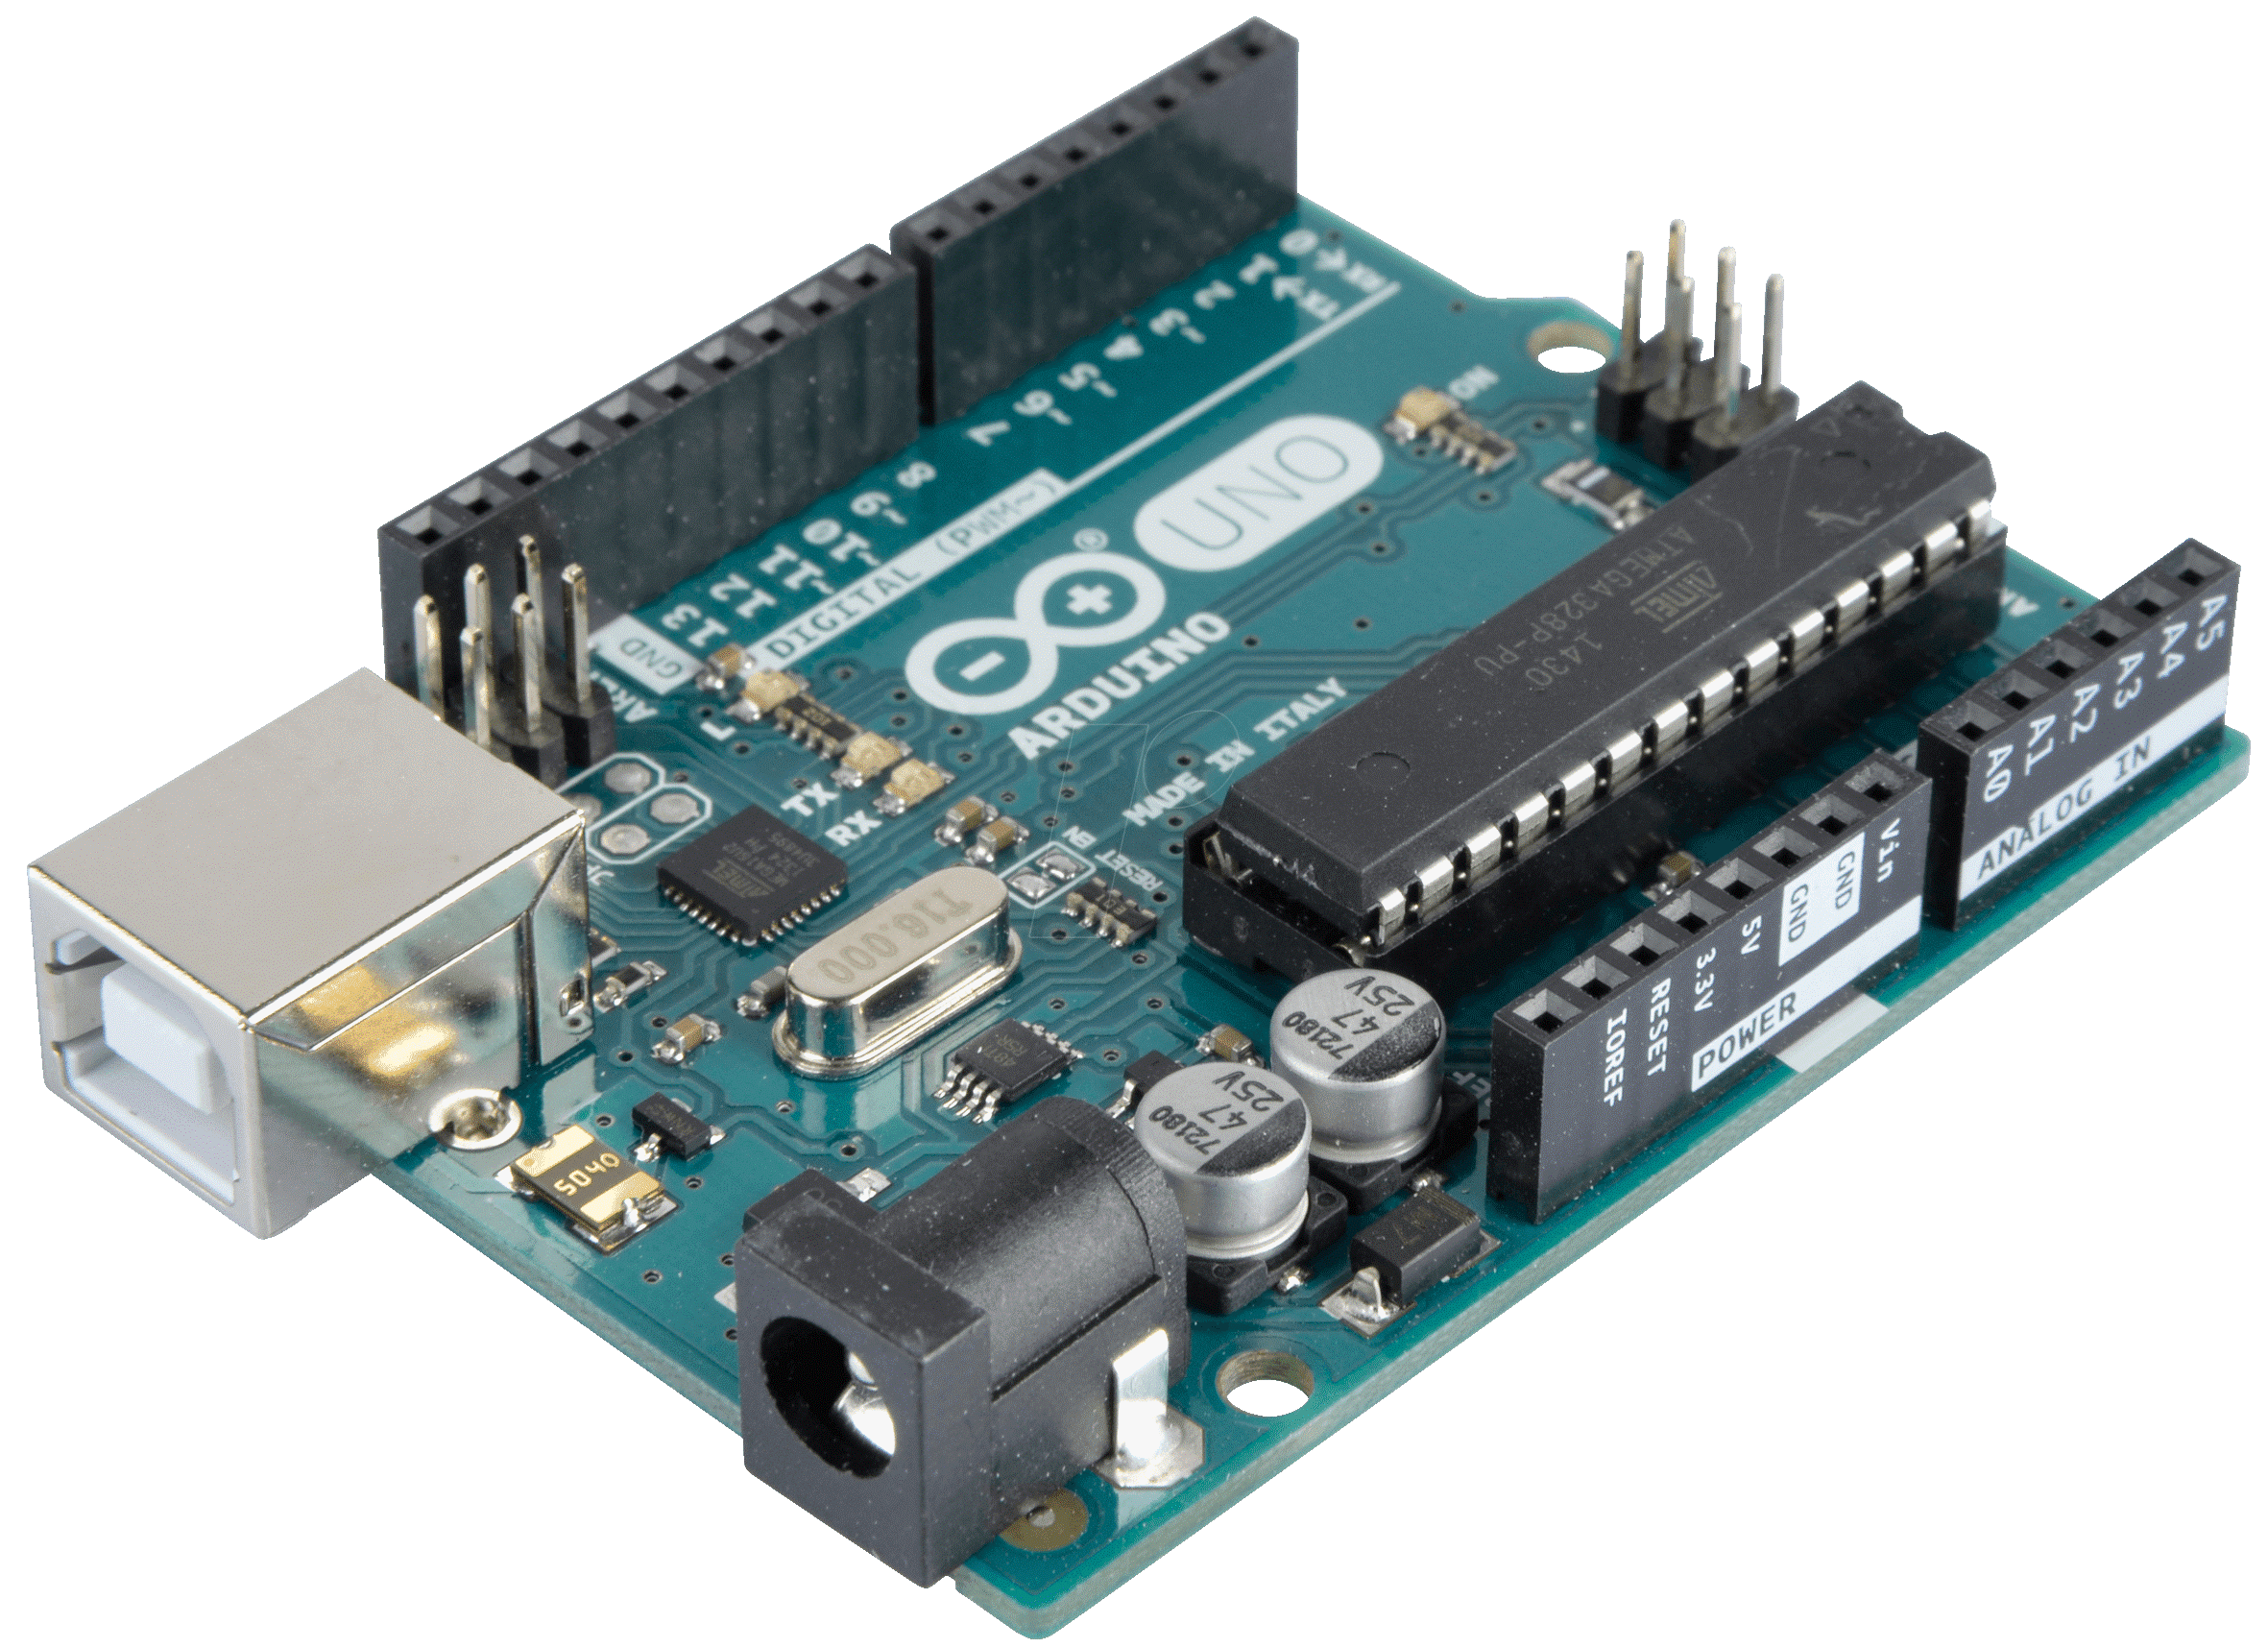
\includegraphics[height= 6cm]{ArduinoUno}
	\caption{Arduino UNO Board} \label{fig:arduino}
\end{figure}

The Microcontroller that we are going to use is Arduino UNO since it is a beginner friendly and easily to code. Arduino UNO, operating at 5V, comes with 14 Digital input and 6 Analog input which is more than enough for this project. Using Arduino UNO make us applied what we have learned so far in the classroom into the real world. Furthermore, Arduino UNO are used in various of projects around the world so that we can have many references and support as we want. We use Arduino UNO to be the main controller.\\

\bfseries{The table of specification}

\begin{table}[H]
	\centering
	\label{tab:arduino}
	\caption{The table of specification of Arduino UNO}
	\pgfplotstabletypeset[
	col sep=comma,
	string type,
	every head row/.style = {before row=\toprule ,after row = \midrule},
	every last row/.style ={after row = \bottomrule},
	columns/No./.style={column type = l}]{Arduino.csv}
\end{table}

\end{document}
